% Copyright 2018-2020 ImmortalPharaoh7, Bryce AS202313
%
% This file is part of Latex-For-The-IB.
%
% Latex-For-The-IB is free software: you can redistribute it and/or modify it
% under the terms of the GNU General Public License as published by
% the Free Software Foundation, either version 3 of the License, or
% (at your option) any later version.
%
% Latex-For-The-IB is distributed in the hope that it will be useful, but
% WITHOUT ANY WARRANTY; without even the implied warranty of
% MERCHANTABILITY or FITNESS FOR A PARTICULAR PURPOSE. See the GNU
% General Public License for more details.
%
% You should have received a copy of the GNU General Public License
% along with Latex-For-The-IB. If not, see http://www.gnu.org/licenses/.
%
\section{Writing your documents}
In this section we will focus on the essential tables / graphs you'll need when writing an IA.

\subsection{Tables}
\href{https://www.overleaf.com/learn/latex/Tables}{Overleaf's documentation on tables}
already provides almost everything you need to write a table.
\href{https://www.tablesgenerator.com/}{This website} generates \LaTeX{} tables
if you would like some sort of GUI assistance when dealing with tables.
But this guide is to offer boilerplate, so here's one for raw data tables
(note: this boilerplate requires the inclusion of the packages mentioned in packages section):
\begin{verbatim}
\begin{table}[H]
\begin{tabu} to \textwidth {X[c]X[c]X[c]X[c]X[c]X[c]X[c]X[c]}
\hline
\multirow{2}{*}{\parbox{2cm}{IV}}&
\multicolumn{6}{c}{DV} \\
\cline{2-8}
& Trial 1 & Trial 2 & Trial 3 & Trial 4 & Trial 5 & Average & Uncert \\
\hline
value & value & value & value & value & value & value & value \\
 & & & & & & & \\
 & & & & & & & \\
 & & & & & & & \\
 & & & & & & & \\
\hline
\end{tabu}
\caption{Table caption}
\end{table}
\end{verbatim}
Resulting table:
\begin{table}[H]
\begin{tabu} to \textwidth {X[c]X[c]X[c]X[c]X[c]X[c]X[c]X[c]}
\hline
\multirow{2}{*}{\parbox{2cm}{IV}}&
\multicolumn{6}{c}{DV} \\
\cline{2-8}
& Trial 1 & Trial 2 & Trial 3 & Trial 4 & Trial 5 & Average & Uncert \\
\hline
value & value & value & value & value & value & value & value \\
 & & & & & & & \\
 & & & & & & & \\
 & & & & & & & \\
 & & & & & & & \\
\hline
\end{tabu}
\caption{Table caption}
\end{table}

Just note that tables are highly customizable and we highly recommend
that you read Overleaf's guide as it will allow you to better understand the code we've used.

\subsection{Graphs}
Now this part has been up for debate for a long time.
There are 2 main approaches on how to implement graphs.
You either can just take a screenshot from Excel or some other software,
or you can use the pgfplots package.
Screenshotting a graph is the fast way which doesn't require a lot of effort
and we recommend doing this if you're short on time.
The other approach takes more time and effort but it's more aesthetically pleasing.
Anyways it's up to you to choose and it's normal if you want to just screenshot and save some time and effort.
However, if you have some time on your hand, we recommend using pgfplots to make your graphs.

\href{https://www.overleaf.com/learn/latex/Pgfplots_package}{Here's the guide that Overleaf wrote}
about the package which we recommend that you read in order to get an idea on how to manipulate the code.
The approach that we're taking is to use Excel in order to get the best fit line / equation,
then we graph the points and just add the best fit its own plot.
Now here's the boilerplate for a non-linear relation graph:

\begin{verbatim}
\begin{figure}[H]
\caption{Graph title}
\begin{center}
\begin{tikzpicture}
\begin{axis}[
    axis lines = left,
    xlabel = X label,
    ylabel = Y label,
    xmin=0, xmax=0.9,
    ymin=1.030, ymax=1.07,
    xtick={0, 0.2, 0.4, 0.6, 0.8},
    ytick={1.03, 1.04, 1.05, 1.06, 1.07},
    legend pos=north west,
]
\addplot [
    domain=0.05:0.8, 
    samples=50, 
    color=blue,
]
{0.0095*ln(x)+1.0667};
 
\addplot[
    only marks,
    color=blue,
    mark=*,
    error bars/.cd,
    y dir=both, y explicit,
    x dir=both, x explicit,
    ]
    coordinates {
    (0.05, 1.0384) +- (0.00204, 0.0015)
    (0.1, 1.0444) +- (0.00315 , 0.0015)
    (0.2, 1.0518) +- (0.00657, 0.001)
    (0.4, 1.0578) +- (0.0148, 0.0015)
    (0.8, 1.0646) +- (0.0563, 0.001)
    };
\end{axis}
\end{tikzpicture}
\end{center}
\end{figure}
\end{verbatim}

\begin{figure}[H]
\caption{Graph title}
\begin{center}
\begin{tikzpicture}
\begin{axis}[
    axis lines = left,
    xlabel = X label,
    ylabel = Y label,
    xmin=0, xmax=0.9,
    ymin=1.030, ymax=1.07,
    xtick={0, 0.2, 0.4, 0.6, 0.8},
    ytick={1.03, 1.04, 1.05, 1.06, 1.07},
    legend pos=north west,
]
\addplot [
    domain=0.05:0.8, 
    samples=50, 
    color=blue,
]
{0.0095*ln(x)+1.0667};
 
\addplot[
    only marks,
    color=blue,
    mark=*,
    error bars/.cd,
    y dir=both, y explicit,
    x dir=both, x explicit,
    ]
    coordinates {
    (0.05, 1.0384) +- (0.00204, 0.0015)
    (0.1, 1.0444) +- (0.00315 , 0.0015)
    (0.2, 1.0518) +- (0.00657, 0.001)
    (0.4, 1.0578) +- (0.0148, 0.0015)
    (0.8, 1.0646) +- (0.0563, 0.001)
    };
\end{axis}
\end{tikzpicture}
\end{center}
\end{figure}

Now the linear graphs are a bit longer than that,
since you have to add minimum and maximum slope along with their equations.
We take the same idea as non linear graphs and apply it,
but this time you don't really need to plot the linear function of the min and max slopes;
you can just connect the 2 points that you use to get the equation.
You're still going to need to add the equations of those in the legend section though.
Here's the boilerplate:

\begin{verbatim}
\begin{figure}[H]
\caption{Graph title}
\begin{center}
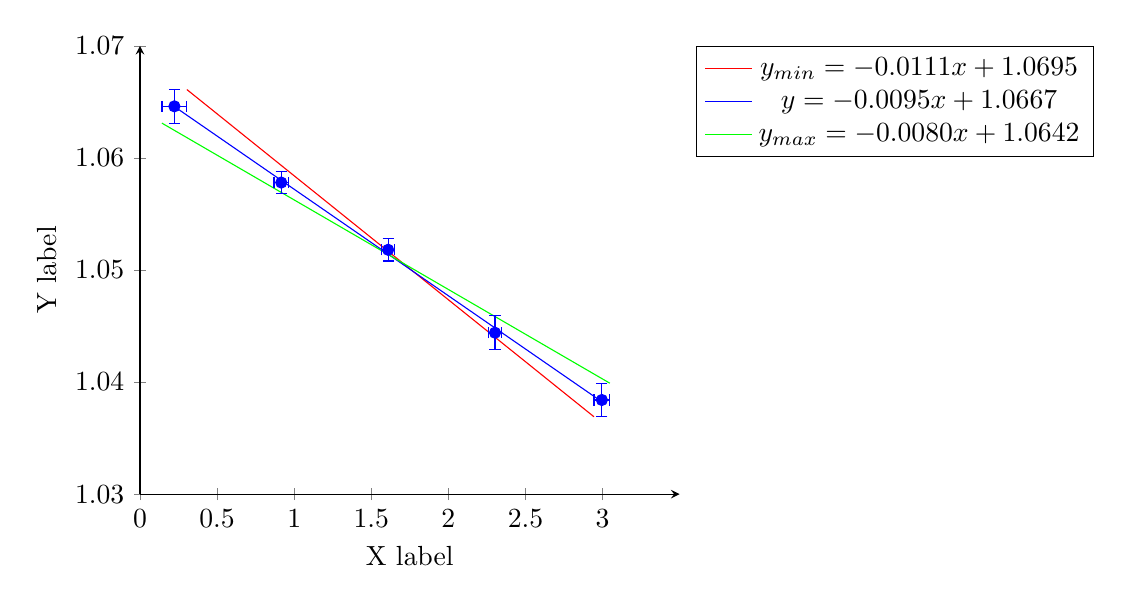
\begin{tikzpicture}
\begin{axis}[
    axis lines = left,
    xlabel = X label,
    ylabel = Y label,
    xmin=0, xmax=3.5,
    ymin=1.030, ymax=1.07,
    xtick={0, 0.5, 1, 1.5, 2, 2.5, 3},
    ytick={1.03, 1.04, 1.05, 1.06, 1.07},
    legend pos=outer north east,
]

\addplot [
    color=red,
]
coordinates {
 (0.3039, 1.0661) (2.9446, 1.0369)
};
\addlegendentry{$y_{min}=-0.0111x+1.0695$}

\addplot [
    domain=0.2231:2.9957, 
    samples=100, 
    color=blue,
]
{-0.0095*x + 1.0667};
\addlegendentry{$y=-0.0095x+1.0667$}

\addplot [
    color=green,
]
coordinates {
(0.1424, 1.0631) (3.0468, 1.0399)
};
\addlegendentry{$y_{max}=-0.0080x+1.0642$}
 
\addplot[
    only marks,
    color=blue,
    mark=*,
    error bars/.cd,
    y dir=both, y explicit,
    x dir=both, x explicit,
    ]
    coordinates {
    (0.2231, 1.0646) +- (0.0807, 0.0015)
    (0.9163, 1.0578) +- (0.0472, 0.001)
    (1.6094, 1.0518) +- (0.0430, 0.001)
    (2.3026, 1.0444) +- (0.0417, 0.0015)
    (2.9957, 1.0384) +- (0.0511, 0.0015)
    };
\end{axis}
\end{tikzpicture}
\end{center}
\end{figure}
\end{verbatim}

\begin{figure}[H]
\caption{Graph title}
\begin{center}
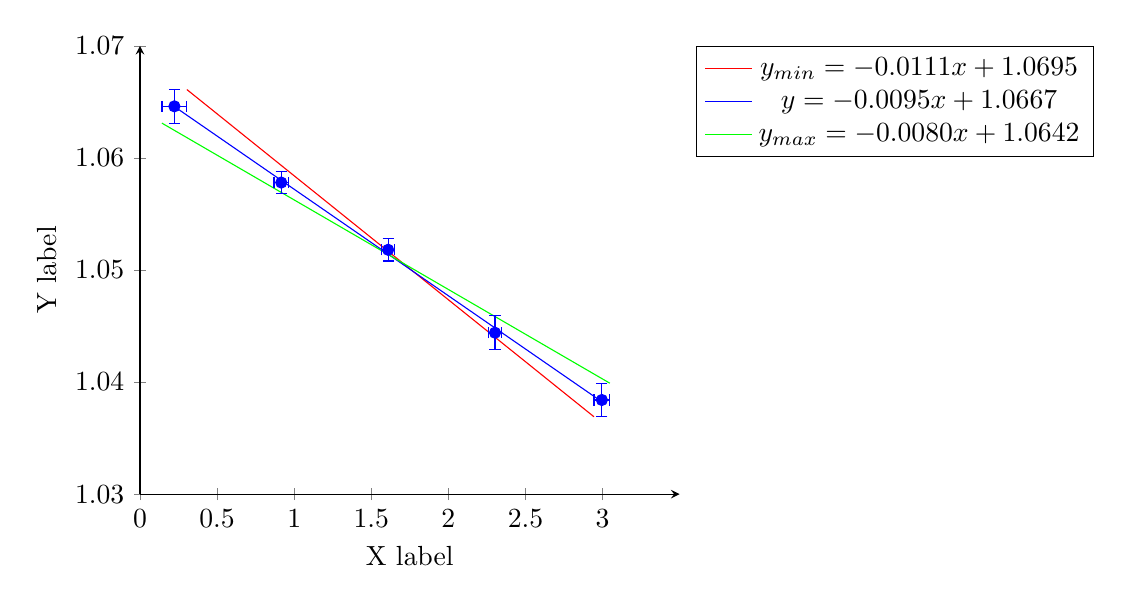
\begin{tikzpicture}
\begin{axis}[
    axis lines = left,
    xlabel = X label,
    ylabel = Y label,
    xmin=0, xmax=3.5,
    ymin=1.030, ymax=1.07,
    xtick={0, 0.5, 1, 1.5, 2, 2.5, 3},
    ytick={1.03, 1.04, 1.05, 1.06, 1.07},
    legend pos=outer north east,
]

\addplot [
    color=red,
]
coordinates {
 (0.3039, 1.0661) (2.9446, 1.0369)
};
\addlegendentry{$y_{min}=-0.0111x+1.0695$}

\addplot [
    domain=0.2231:2.9957, 
    samples=100, 
    color=blue,
]
{-0.0095*x + 1.0667};
\addlegendentry{$y=-0.0095x+1.0667$}

\addplot [
    color=green,
]
coordinates {
(0.1424, 1.0631) (3.0468, 1.0399)
};
\addlegendentry{$y_{max}=-0.0080x+1.0642$}
 
\addplot[
    only marks,
    color=blue,
    mark=*,
    error bars/.cd,
    y dir=both, y explicit,
    x dir=both, x explicit,
    ]
    coordinates {
    (0.2231, 1.0646) +- (0.0807, 0.0015)
    (0.9163, 1.0578) +- (0.0472, 0.001)
    (1.6094, 1.0518) +- (0.0430, 0.001)
    (2.3026, 1.0444) +- (0.0417, 0.0015)
    (2.9957, 1.0384) +- (0.0511, 0.0015)
    };
\end{axis}
\end{tikzpicture}
\end{center}
\end{figure}

\subsection{BibLaTeX}